% Horizon penetrating coordinates (vs. Schwarzschild coordinates)
% for a black hole spacetime, with excision
% Author: Jonah Miller
\documentclass[tikz,border=6pt]{standalone}
\usepackage{tikz}
\usetikzlibrary{arrows}
\usetikzlibrary{arrows.meta}
\usetikzlibrary{decorations.markings}
\usepackage{pgfplots}

%\tikzset{>={Latex[length=3mm]}}

\begin{document}
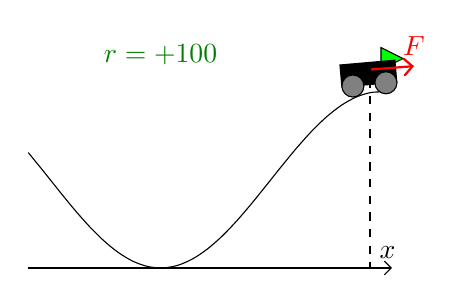
\begin{tikzpicture}[scale=1.4]

\def\flagheight{4/5}
\def\carlength{0.3}

\draw[scale=1,domain=0.8:4.05,smooth,variable=\x] plot ({\x},{\flagheight*cos(90*\x)});

\draw[-,fill=green] (4,\flagheight) -- (4,{\flagheight + 0.4}) -- (4.2,{\flagheight + 0.3}) -- (4,{\flagheight+0.2});


\def\carx{3.8}
\def\cary{\flagheight*cos(90*\carx)}
\def\carytwo{\flagheight*cos(90*(\carx+\carlength))}

\def\deltax{-0.055}
\def\deltay{0.09}

\draw[-,fill=black,rotate around={5:({\carx+\deltax},{\cary+\deltay})}] ({\carx+\deltax-0.1},{\cary+\deltay}) rectangle({\carx+\deltax+0.4},{\cary+\deltay+0.2});
\draw[-,fill=gray] ({\carx+\deltax},{\cary+\deltay}) circle(0.1);
\draw[-,fill=gray] ({\carx+\carlength+\deltax},{\carytwo+\deltay}) circle(0.1);

\draw[thick, red, -angle 90] (3.9,1) -- (4.3,1.031) node[above]{$F$};

\draw[black!50!green](2,1.13) node{$r=+100$};

%\draw[-angle 90,thick] (0.8,{-\flagheight}) -- (4.1,{-\flagheight}) node[above=6pt,left=0.5pt]{$x$};

\draw[-angle 90] (0.8,{-\flagheight}) -- (4.1,{-\flagheight});% node[above]{$x$};
\draw[dashed] ({\carx+0.1},{\cary+0.3}) -- ({\carx+0.1}, {-\flagheight}) node[above right]{$x$};

\end{tikzpicture}
\end{document}